\documentclass[a4paper,10pt]{scrartcl}
\usepackage[utf8]{inputenc}
\usepackage[ngerman]{babel}
\usepackage[T1]{fontenc}
\usepackage{booktabs}
\usepackage{xspace}
\usepackage{enumitem}
\usepackage{cite}
\usepackage{graphicx}
\usepackage{tikz}
\usetikzlibrary{arrows}
\usetikzlibrary{fit}
\usetikzlibrary{calc}
\usepackage{float}
\usepackage[section]{placeins} % don't move figures beyond the next section heading

% this is needed for forms and links within the text
\usepackage{hyperref}

% glossary, see http://en.wikibooks.org/wiki/LaTeX/Glossary
% has to be loaded AFTER hyperref so that entries are clickable
\usepackage[nonumberlist]{glossaries}

\makeglossary

% Variables
\newcommand{\authors}{
   Mohammed~Abu~Jayyab,
   Niklas~Baumstark,
   Tobias~Gräf,
   Amrei~Loose\xspace
}
\newcommand{\authorName}{ \authors, Christoph~Michel }
\newcommand{\authorNameEmph}{ \authors, \textbf{Christoph~Michel} }

\newcommand{\dateFirstVersion}{\today}
\newcommand{\customer}{Karlsruher Institut für Technologie}
\newcommand{\contractor}{Eine Firma}
\newcommand{\projectName}{Broadcast-Verschlüsselung\xspace}
\newcommand{\tags}{
   \authorName,
   Pflichtenheft,
   KIT,
   Informatik,
   PSE,
   Broadcast-Verschlüsselung
}
\newcommand{\glossarName}{Glossar}
\newcommand{\doctitle}{\projectName (Pflichtenheft)}
\title{\doctitle}
\author{\authorName}
\date{\today}

% less margin
\usepackage[margin=2.5cm]{geometry}

% horizontal line
\newcommand{\HRule}{\rule{\linewidth}{0.5mm}}

% more beautiful lists
\setlist{noitemsep}
\renewcommand{\labelitemi}{$\bullet$}
\renewcommand{\labelitemii}{$\diamond$}

% create a shorter version for tables
\newcommand\addrow[2]{#1 &#2\\ }
\newcommand\addheading[2]{\textbf{\sffamily #1} &\textbf{\sffamily #2}\\ \hline}
\newcommand\tabularhead{\begin{tabular}{lp{13cm}}
\hline
}

\newcommand\addmulrow[2]{ \begin{minipage}[t][][t]{2.5cm}#1\end{minipage}%
   &\begin{minipage}[t][][t]{8cm}
    \begin{enumerate} #2   \end{enumerate}
    \end{minipage}\\ }

\newenvironment{usecase}{\tabularhead}
{\hline\end{tabular}}

% a cross
\newcommand\X{$\times$}

% templates and default styles for figures and graphics
\tikzset{>=triangle 45}
\tikzset{font=\sffamily}

\newcommand{\tmpCaption}{}
\newenvironment{illustration}[1]
{
   \renewcommand{\tmpCaption}{#1}
   \begin{figure}[h!]
   \centering
}
{
   \caption{\tmpCaption}
   \end{figure}
}


\begin{document}

\maketitle
  \begin{tabular}[t]{ll}
	Projekt:       & \quad \projektName \\[1.2ex]
	Auftraggeber:  & \quad \auftraggeber\\[1.2ex]
	Auftragnehmer: & \quad \auftragnehmer\\[1.2ex]
  \end{tabular}

\begin{tabular}{|p{3 cm}|p{3 cm}|p{5 cm}|}
\hline
\textbf{Version} & \textbf{Datum} & \textbf{Autor(en)} \\
\hline
\hline
1.0 & 29.04.2012 & \authorName \\
\hline
\end{tabular}

\tableofcontents
\clearpage

\section{Einleitung}

Heutzutage gängige Streamingdienste im Internet basieren bis auf wenige Ausnahmen auf
einem Client-Server-Modell, bei dem jeder Client eine eigene Verbindung zum Server
aufbaut, um einen Stream zu empfangen. Das Trafficaufkommen, das durch diese Art der
Kommunikation verursacht wird sowie die notwendige Bandbreite sind enorm. Nur große
Anbieter von Inhalten können sich diese Form der Verteilung überhaupt leisten.

Mit der naheliegenden Erkenntnis, dass bei dem beschriebenen Verfahren dieselben Daten
vielfach an verschiedene Empfänger versendet werden, ergibt sich ein alternatives
Vorgehen auf der Basis von Multicast: Inhalte werden vom Server nur einmal versendet
und über das Internet an mehrere Empfänger zugestellt. Damit wird vor allem der Sender,
aber auch die gesamte Internet-Infrastruktur entlastet.

Ein großes Problem stellt allerdings die Zugangskontrolle für diese Multicast-Streams
dar: Da nun der Server nicht mehr weiß, wer eigentlich den Stream empfängt, kann
er auch nicht verhindern, dass unauthorisierte Benutzer Zugang erhalten. Die Lösung
dieses Problems erfordert den Einsatz von speziellen Verschlüsselungsverfahren,
sodass zwar jeder den Stream empfangen, aber nur authorisierte Benutzer den Stream
entschlüsseln können. Besonderes Augenmerk muss dabei auf Effizienz gelegt werden,
da der Kommunikationsaufwand durch die Verschlüsselung nicht wesentlich erhöht werden
darf.

Wir wurden daher beauftragt, einen Prototyp zu entwickeln, der ein
Broadcast"=Verschlüsselungsverfahren mit speziellen wünschenswerten Eigenschaften
demonstriert.

\section{Zielbestimmung}

Die entwickelte Software ist eine Client/Server-Kombination, die es ermöglicht,
Inhalte verschlüsselt von einem Server an verschiedene Clients verteilen. Dafür
soll kein bidirektionales Kommunikationsmedium erforderlich sein.

Die Clients werden auf Basis des g"angigen mobilen Betriebssystems Android
implementiert.

Es wird ein Verschlüsselungsverfahren eingesetzt, welches die besondere
Eigenschaft besitzt, nicht mit der Gesamtzahl der Empfänger, sondern mit der Anzahl
ausgeschlossener Benutzer zu skalieren.

\subsection{Musskriterien}

\begin{itemize}

\item Server
\begin{itemize}
   \item sendet Daten an eine Empfängergruppe. Zu Demonstrationszwecken wird
         ein einfacher Audio- oder Videostream als Payload eingesetzt.
   \item erlaubt es, nicht mehr authorisierte Benutzer auszuschließen.
\end{itemize}

\item Client
\begin{itemize}
   \item erlaubt es, sich mit einem Server zu verbinden (einer Gruppe beizutreten).
   \item empfängt Daten vom Server und stellt sie dar.
   \item merkt sich zuletzt ausgew"ahlte Server, sodass ein erneuter Zugriff schnell
         m"oglich ist.
\end{itemize}

\item Kommunikation und Verschl"usselung
\begin{itemize}
   \item Nur ein unidirektionaler Kommunikationskanal vom Server zum Client wird
         vorausgesetzt. Zu Demonstrationszwecken wird TCP als Transportprotokoll
         verwendet, aber auch zuverl"assige Multicastprotokolle k"amen als Medium
         infrage.
   \item Daten werden verschl"usselt "ubertragen. Der Server bietet entsprechende
         Optionen zur Erzeugung von Schl"usseln und zur Kontrolle und Konfiguration
         der Verschl"usselungsschicht. "Uber einen externen, sicheren Kanal erh"alt
         jeder Benutzer einen privaten Schl"ussel (z.B. eine Datei), mit dem er seine
         Clientsoftware konfigurieren kann.
   \item Das verwendete Broadcast"=Verschl"usselungsverfahren basiert auf den
         in~\cite[Section~2.2]{Naor00} oder~\cite{Garg10} beschriebenen Verfahren
         oder einer Variante der Algorithmen mit vergleichbaren kryptografischen
         Eigenschaften.
   \item Die Verschl"usselung erfordert im laufenden Betrieb nur einen
         Kommunikationsoverhead, der sublinear in der Gesamtanzahl der Benutzer und
         stattdessen linear oder quasilinear in der Anzahl der ausgeschlossenen
         Benutzer ist.
\end{itemize}
\end{itemize}

\subsection{Wunschkriterien}

\begin{itemize}

\item Server
\begin{itemize}
   \item f"uhrt Statistik "uber Nutzdatenmenge und Traffic, um den Kommunikationsaufwand
         der Verschl"usselung zu analysieren.
   \item Gesperrte Benutzer lassen sich wieder entsperren
\end{itemize}

\item Client
\begin{itemize}
   \item verf"ugt "uber eine Anzeige des angefallenen Traffics.
   \item puffert oder speichert Inhalte, sodass z.B. in einem Stream auch
         zur"uckgespult werden kann.
\end{itemize}

\item Kommunikation und Verschl"usselung
\begin{itemize}
   \item Die Verbindung des Clients zum Server erfolgt ohne eine zus"atzliche TCP-Verbindung.
         Dazu muss ein Verfahren entwickelt werden, bei dem der Server den Session-Key
         in regelm"a"sigen Abst"anden sendet.
   \item Ein effizienteres Verfahren als das in~\cite{Naor00} beschriebene wird
         entwickelt und implementiert.
\end{itemize}
\end{itemize}

\subsection{Abgrenzungskriterien}
\begin{itemize}
   \item Es wird kein Framework zur Verf"ugung gestellt, welches verschiedene
         Streamtypen implementiert. Stattdessen bleibt die Implementierung
         unabh"angig von den zugrundeliegenden Nutzdaten und ist so flexibel,
         dass eine konkrete Implementierung eines neuen Streamtyps problemlos
         m"oglich ist.
   \item Es wird kein Multicast-Protokoll implementiert. Stattdessen wird
         zur Demonstrationszwecken TCP zur Kommunikation benutzt und die Software
         ist so flexibel, dass eine Adaptation an ein zuverl"assiges
         Multicastverfahren problemlos m"oglich ist.
\end{itemize}

\section{Produkteinsatz}

Das Produkt wird benutzt um Inhalte an eine festgelegte Benutzergruppe zu verteilen. 

\subsection{Anwendungsbereich}

Durch die Abstraktion vom gesendeten Datentyps kann das Produkt in allen Bereichen zum Einsatz kommen,
die das Verteilen von Daten an bestimmte Nutzergruppen erfordern, z.B. f"ur Media-Streaming oder
die Verteilung von Texten und Bildern.

Da das Verfahren eine sehr breite Verteilung erm"oglicht, bietet es sich unter anderem für das
Live-Streaming bedeutender Events an. Dabei kommt es aufgrund großen "offentlichen Interesses
häufig zur Überlastung der Server, was mithilfe der entwickelten Software umgangen werden k"onnte.

Mithilfe der Verschl"usselung kann das Programm auch für kostenpflichtige Internetdienste
wie Pay-TV, Zeitschriften, etc. verwendet werden.

\subsection{Zielgruppen}

Es gibt in diesem Fall zwei Zielgruppen: Die der Dienstanbieter und die der Nutzer.

Die Dienstanbieter sind die Betreiber der Server, die Inhalte an die Nutzer verteilen wollen. Sie
möchten die Möglichkeit einer Zugangskontrolle zu ihrem Dienst haben.

Die Nutzer wollen die Dienstleistung in Anspruch nehmen und Daten empfangen.

\subsection{Betriebsbedingungen}

Der Server läuft im unbeaufsichtigten, stationären Dauerbetrieb.

Der Client wird mobil und nur auf Anfrage benötigt.

\section{Produktumgebung}

Der Server muss auf einem Java-fähigen System laufen.
Der Client muss auf einem portablen Gerät auf Basis des Android-Betriebssystems laufen.

\subsection{Software}
\begin{itemize}
\item Client
   \begin{itemize}
      \item Betriebssystem: Android (mindestens 2.1)
   \end{itemize}
\item Server
   \begin{itemize}
      \item Java-fähiges System
   \end{itemize}
\end{itemize}

\subsection{Hardware}
\begin{itemize}
\item Client
   \begin{itemize}
      \item Internetfähiges Smartphone mit folgenden Mindestanforderungen:
         \begin{itemize}
         \item 500 MHz CPU
         \item 384 MB RAM
         \item 240$\times$320 Pixel Displayaufl"osung
      \end{itemize}
   \end{itemize}
\item Server
   \begin{itemize}
      \item Angemessene Hardwareausstattung, je nach Auslastung des Dienstes und
            Anzahl der Benutzer.
   \end{itemize}
\end{itemize}

\section{Produktfunktion}

\subsection{Grundfunktionen}

\begin{usecase}
\addheading{Nummer}{Beschreibung}
\addrow{/FA10/} {Der Server versendet Daten an eine Empf"angergruppe.}
\addrow{/FA20/} {Der Server bietet die M"oglichkeit einer initialen Schl"usselerzeugung, wobei
                 ein kompletter Satz privater Schl"ussel f"ur die Benutzer erstellt wird.
                 Diese m"ussen dann auf einem sicheren Weg zugestellt werden.}
\addrow{/FA30/} {Der Server verschl"usselt Daten so, dass nur authorisierte
                 Benutzer den Stream entschl"usseln k"onnen.}
\addrow{/FA40/} {Der Server bietet die M"oglichkeit, Nutzer per Namen auszuschließen,
                 ohne dass eine neue Schl"usselerzeugung erforderlich ist.}
\addrow{/FA50/} {Der Client bietet die M"oglichkeit, sich zu einem Server verbinden.}
\addrow{/FA60/} {Der Client empf"angt Daten und stellt sie dar.}
\addrow{/FA70/} {Der Client erlaubt die Angabe eines privaten Schl"ussels, der von
                 einem Server erzeugt wurde.}
\addrow{/FA80/} {Der Client kann Daten entschlüsseln, nachdem er mit einem
                 g"ultigen Schl"ussel konfiguriert wurde und solange er nicht
                 vom Server explizit ausgeschlossen wurde.}
\addrow{/FA90/} {Der Client merkt sich den letzten ausgewählten Server mit
                 zugeh"origem Schl"ussel, sodass ein erneuter Zugriff schnell möglich
                 ist.}
\addrow{/FA100/} {Die Verschlüsselung erfolgt mit einer Variante des in~\cite[Section 2.2]{Naor00}
                  oder~\cite{Garg10} vorgestellten Verfahrens}
\end{usecase}

\subsection{Erweiterte Funktionen}

\begin{usecase}
\addheading{Nummer}{Beschreibung}
\addrow{/FA200/} {Der Benutzer kann im Client mehrere Serverfavoriten
                  mit Namen und Schl"usseln in einem dedizierten Optionsdialog verwalten,
                  welche dann über ein Kontextmenü auswählbar sind.}
\addrow{/FA210/} {Der Server führt Statistiken über Nutzdatenmenge und Traffic,
                  um den Kommunikationsaufwand für die Verschlüsselung zu
                  analysieren}
\addrow{/FA220/} {Der Server bietet die M"oglichkeit, ausgeschlossene Benutzer wieder
                  zu authorisieren.}
\addrow{/FA230/} {Der Client verfügt über eine Anzeige des angefallenen Traffics.}
\addrow{/FA240/} {Der Client verfügt über eine Anzeige des angefallenen Traffics.}
\addrow{/FA250/} {Um Benutzer mit volumenbasierten Datentarifen nicht zu belasten,
                  bietet der Client einen WiFi-Modus, in dem er nur bei
                  verf"ugbarer drahtloser Netzwerkverbindung eine Verbindung erlaubt,
                  und nicht "uber das Telefonanbieternetz.}
\addrow{/FA260/} {Der Client puffert empfangene Daten, um eine flüssigere
                  Wiedergabe zu ermöglichen.}
\addrow{/FA270/} {Ein effizienteres Verschlüsselungsverfahren als das in~\cite{Naor00} beschriebene
                  wird verwendet.}
\end{usecase}

\section{Produktdaten}
Da die Software nicht f"ur die Kundenverwaltung des Anbieters zust"andig ist, werden keine
konkreten Benutzerdaten gespeichert. Stattdessen bleibt die Erfassung und Haltung der Daten
dem Anbieter "uberlassen und lediglich ein Identifikationsstring wird im Server direkt gespeichert.

\subsection{Grunddaten}
\begin{usecase}
\addheading{Nummer}{Beschreibung}
\addrow{/PD10/} {Server: Benutzerdaten
   \begin{itemize}
   \item User-ID (beliebiger String)
   \item Privater Schl"ussel
   \item Status: ausgeschlossen oder authorisiert
   \end{itemize}
}
\addrow{/PD20/} {Client: Daten des zuletzt besuchten Servers
   \begin{itemize}
   \item Hostname/Port-Kombination
   \item Privater Schl"ussel
   \end{itemize}
}
\end{usecase}

\subsection{Erweiterte Daten}
\begin{usecase}
\addheading{Nummer}{Beschreibung}
\addrow{/PD30/} {Server/Client: Trafficstatistiken
   \begin{itemize}
   \item "ubertragene/empfangene Nutzdatenmenge
   \item "ubertragene/empfangene Datenmenge insgesamt
   \end{itemize}
}
\addrow{/PD40/} {Client: Liste von Servern
   \begin{itemize}
   \item (optional) Alias
   \item Hostname/Port-Kombination
   \item Privater Schl"ussel
   \end{itemize}
}
\end{usecase}

\section{Systemmodell}

\begin{illustration}{Client/Server-Modell unserer Broadcasting-Anwendung}

\tikzset{
  rect/.style={draw,fill=green!15,minimum height=0.8cm,rectangle},
  box/.style={
    draw=blue!50!white,
    line width=1pt,
    dash pattern=on 1pt off 4pt on 6pt off 4pt,
    inner sep=4mm, rectangle, rounded corners
  },
}

\begin{tikzpicture}[auto,node distance=1.5cm]

\node[rect](server) {\textbf{Server}};
\node[rect,minimum width=2cm,xshift=5cm,right of=server](view) {View};
\node[rect,minimum width=2cm,below of=view](controller) {Controller};
\node[box,fit=(view.north west) (view.north east)
              (controller.south east) (controller.south west),
      inner sep=0.3cm](client) {};

\node[rect,fill=red!15,below of=client,xshift=-3cm,yshift=-2cm](library)
    {\textbf{Broadcast-Library}};
\node at (client.north) [above, inner sep=2mm] {\textbf{Client}};

\draw [->] (server.east) -- (client.west |- server.east)
           node[pos=.5]{sendet an}
           node[pos=0.94]{*};

%\path[->] (server) edge node {sendet an *} (client);
\path[->] (view) edge node {} (controller);
\path[->] (controller) edge node {} (view);
\path[->] (controller) edge node {benutzt} (library);
\path[->] (server) edge node {benutzt} (library);

\end{tikzpicture}

\end{illustration}

\begin{illustration}{Kommunikations-Modell unserer Broadcasting-Anwendung}

\tikzset{
  rect/.style={draw,fill=green!15,minimum height=0.8cm,rectangle},
  box/.style={
    draw=blue!50!white,
    line width=1pt,
    dash pattern=on 1pt off 4pt on 6pt off 4pt,
    inner sep=4mm, rectangle, rounded corners
  },
}

\begin{tikzpicture}[auto,node distance=1.5cm]

\node[rect,minimum width=2cm](server) {\textbf{Server}};
\node[rect,minimum width=2cm,xshift=4.5cm,right of=server](client) {Client};

\node[rect,minimum width=2cm, fill=red!15, below of=server](dataleft) {\textbf{}};
\node[rect,minimum width=2cm, fill=red!15, below of=client](dataright) {\textbf{}};

\node[box,fit=(dataleft.north west) (dataright.north east)
              (dataright.south east) (dataleft.south west),
      inner sep=0.3cm](data) {};

\node at (dataleft.east) [right, inner sep=1cm] {\textbf{Nutzdaten}};

\node[rect,minimum width=2cm, fill=red!15, below of=dataleft](encleft) {\textbf{}};
\node[rect,minimum width=2cm, fill=red!15, below of=dataright](encright) {\textbf{}};

\node at (encleft.east) [right, inner sep=1cm] {\textbf{Verschlüsselung}};

\node[box,fit=(encleft.north west) (encright.north east)
              (encright.south east) (encleft.south west),
      inner sep=0.3cm](encryption) {};

\node[rect,minimum width=2cm, fill=red!15, below of=encleft](transpleft) {\textbf{}};
\node[rect,minimum width=2cm, fill=red!15, below of=encright](transpright) {\textbf{}};

\node[box,fit=(transpleft.north west) (transpright.north east)
              (transpright.south east) (transpleft.south west),
      inner sep=0.3cm](transport) {};

\path[->]
  (server) edge node {} (dataleft)
  (dataleft) edge node {} (encleft)
  (encleft) edge node {} (transpleft)
  (transpright) edge node {} (encright)
  (encright) edge node {} (dataright)
  (dataright) edge node {} (client)
  
  
  ;
\path[<->]
   (transpleft) edge node{Transport} (transpright)
  ;
  ;

\end{tikzpicture}

\end{illustration}
\begin{illustration}{Nutzer können entweder die Daten entschlüsseln(grün) oder sind ausgeschlossen(rot)}

\tikzset{
  rect/.style={draw,fill=green!15,minimum height=0.8cm,rectangle},
  box/.style={
    draw=blue!50!white,
    line width=1pt,
    inner sep=4mm, rectangle, rounded corners
  },
}

\begin{tikzpicture}[auto,node distance=1.5cm]

\node[rect,minimum width=2cm](server) {\textbf{Server}};
\node[rect,minimum width=2cm,xshift=4.5cm,right of=server](client) {\textbf{Client}};

\node[box,fit=(dataleft.north west) (dataright.north east)
              (dataright.south east) (dataleft.south west),
      inner sep=0.2cm](data) {};

\end{tikzpicture}

\end{illustration}


\section{Produktleistung}

\begin{usecase}
\addheading{Nummer}{Beschreibung}
\addrow{/L10/} {Das Verschlüsselungssystem ist in der Lage, 100000 Benutzer zu bedienen,
                wobei h"ochstens 500 Benutzer einen nicht mehr g"ultigen privaten Schl"ussel
                besitzen und daher nicht bedient werden d"urfen.}
\addrow{/L20/} {Die Oberfläche der Client-Anwendung ist so intuitiv, dass jeder Benutzer
                sich innerhalb von höchstens 5 Minuten Einarbeitungszeit selbst
                zurechtfindet, ohne die Dokumentation konsultieren zu müssen.}
\addrow{/L30/} {Die Antwort auf einen Klick eines Benutzers erfolgt innerhalb von
                höchstens 200ms.}
\addrow{/L40/} {Die Dauer der Anmeldnung muss weniger als 20 Sekunden betragen.}
\addrow{/L50/} {Bei fehlerhaften Eingaben wird dem Benutzer eine entsprechende
                Fehlermeldung angezeigt.}
\addrow{/L60/} {Der Server zeigt korrigierbare Ausnahmesituationen an und loggt diese,
                anstatt sofort abzust"urzen.}
\end{usecase}

\section{GUI}

\begin{illustration}{Der Ausgangsbildschirm, von dem aus es möglicht ist, zu einem Server zu verbinden.}
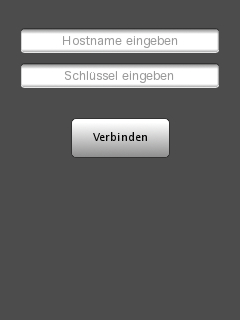
\includegraphics[width=150px]{figures/images/homescreen.jpg}
\end{illustration}
\begin{illustration}{Eine Fehlermeldung nach einer Falscheingabe oder ähnlichem.}
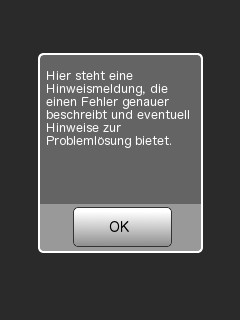
\includegraphics[width=150px]{figures/images/alert.jpg}
\end{illustration}
\begin{illustration}{Der optionale Optionsbildschirm entsprechend den Wunschkriterien.}
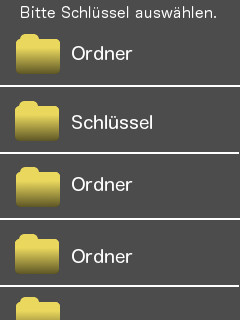
\includegraphics[width=150px]{figures/images/filebrowser.jpg}
\end{illustration}
\begin{illustration}{Der optionale Optionsbildschirm entsprechend den Wunschkriterien.}
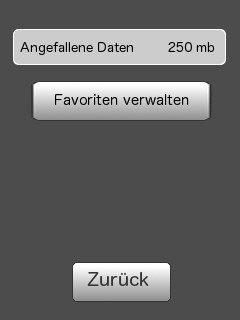
\includegraphics[width=150px]{figures/images/optionscreen.jpg}
\end{illustration}
\begin{illustration}{Eine mögliche Abfolge von Befehlen in der Serverkonsole.}
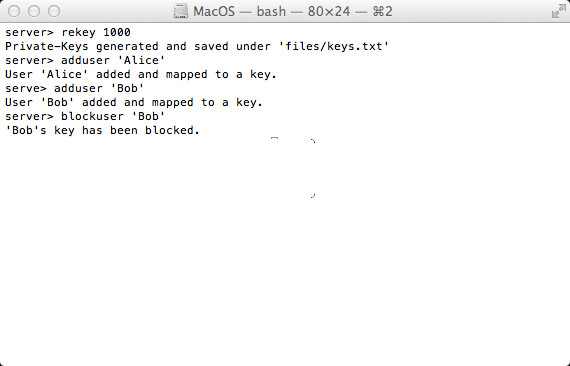
\includegraphics[width=350px]{figures/images/serverterminal.jpg}
\end{illustration}

\section{Testfälle und Testszenarien}

\subsection{Testf"alle}

\begin{usecase}
\addheading{Nummer}{Beschreibung}
\addrow{/TF10/} {Anmeldung durch privilegierten Benutzer
   \begin{itemize}
   \item Teilnehmender Akteur: Benutzer
   \item Eingangsbedingung: Der Benutzer hat seinen Schlüssel erhalten und es werden Daten vom Anbieter
                            gesendet.
   \item Ausgangsaktion: Der Benutzer kann die gewünschten Daten ansehen.
   \item Ereignissfluss: Der Benutzer wird dazu aufgefordert den Anbieter und seinen Schlüssel
         einzugeben. Damit kann er die Daten betrachten, da er nicht explizit ausgeschlossen wurde.
   \end{itemize}
}
\addrow{/TF15/} {Anmeldung durch ausgeschlossenen Benutzer
   \begin{itemize}
   \item Teilnehmender Akteur: Benutzer
   \item Eingangsbedingung: Der Benutzer hat seinen Schlüssel erhalten und wurde ausgeschlossen.
   \item Ausgangsaktion:  Da der Benutzer ausgeschlossen wurde bleibt ihm der Zugang verwehrt und er kann
             die Daten nicht betrachten
   \item Ereignissfluss: Der Benutzer wird dazu aufgefordert den Anbieter und seinen Schlüssel
         einzugeben.Er durch eine Fehlermeldung auf eine eventuelle Falscheingabe aufmerksam gemacht, aber selbst wenn er keinen
         Fehler gemacht hat bleibt ihm der Zugriff verwehrt, da er explizit vom Anbieter ausgeschlossen wurde.
   \end{itemize}
}
\addrow{/TF20/} {Schl"usselerzeugung
   \begin{itemize}
   \item Teilnehmender Akteur: Anbieter
   \item Eingangsbedingung: -
   \item Ausgangsaktion: Ein neues Satz privater Schlüssel wird gespeichert.
   \item Ereignissfluss: Der Anbieter will ein neue Empfängergruppe eröffnen und lässt
         den Server einen neuen Satz privater Schlüssel zur Verteilung erstellen.
   \end{itemize}
}
\addrow{/TF30/} {Starte Datenübertragung
   \begin{itemize}
   \item Teilnehmender Akteur: Anbieter
   \item Eingangsbedingung: Es existiert ein Satz Schl"ussel.
   \item Ausgangsaktion: Benutzer sind in der Lage die gesendeten Inhalte zu empfangen.
   \item Ereignissfluss: Der Anbieter wählt Inhalte aus, die gesendet werden soll, aus und
         teilt diese dem Server mit. Diese Inhalte werden vom Server in verschlüsselter Form
         versendet, so dass ausgeschlossene Nutzer sie nicht entschlüsseln können.
   \end{itemize}
}
\addrow{/TF40/} {Benutzer sperren
   \begin{itemize}
   \item Teilnehmender Akteur: Anbieter
   \item Eingangsbedingung: Es existiert ein Satz Schl"ussel und mindestens ein Benutzer.
   \item Ausgangsaktion: Der betreffende Benutzer kann die Daten nicht mehr entschlüsseln
   \item Ereignissfluss: Der Anbieter teilt dem Server mit welchen Benutzer er ausschließen möchte.
         Die betreffenden Daten werden vom Server gespeichert und die Auswirkungen werden
         sofort sichtbar. Falls der ausgeschlossene Benutzer gerade einen Stream empf"angt,
         erscheint im Client eine Fehlermeldung.
   \end{itemize}
}
% unterbrechen der Tabelle, damit sie über 2 Seiten geht
\end{usecase}
\clearpage
\begin{usecase}

\addrow{/TF50/} {Benutzer hinzufügen
   \begin{itemize}
   \item Teilnehmender Akteur: Anbieter
   \item Eingangsbedingung: Es existiert ein Satz Schl"ussel.
   \item Ausgangsaktion: Der dem Benutzer zugeordnete Schl"ussel wird gespeichert.
   \item Ereignissfluss: Der Anbieter übergibt dem Server die nötigen Daten über den Benutzer.
         Dieser speichert die Informationen und ordnet dem Benutzer einen privaten Schlüssel
         zu, welcher in einer vorgegebenen Datei gespeichert wird.
   \end{itemize}
}

\addrow{/TF60/} {Ungültige Befehle
   \begin{itemize}
   \item Teilnehmender Akteur: Anbieter
   \item Eingangsbedingung: keine
   \item Ausgangsaktion: Es wird eine Fehlermeldung angezeigt.
   \item Ereignissfluss:
          Eine der folgenden Situationen entsteht:
          \begin{itemize}
           \item Der Anbieter startet eine Datenübertragung ohne vorher eine Schl"usselerzeugung
                 durchzuf"uhren
           \item Obwohl keine Schlüsselerzeugung durchgeführt wurde fügt der Anbieter einen Benutzer hinzu.
           \item Ein Benutzer, der nicht existiert, wird vom Anbieter gesperrt.
           \end{itemize}
   \end{itemize}
}
\addrow{/TF70/} {Menschliche Schwäche
   \begin{itemize}
   \item Teilnehmender Akteur: Benutzer
   \item Eingangsbedingung: Vom Anbieter werden Daten gesendet und Benutzer ist authorisiert.
   \item Ausgangsaktion: Benutzer kann Daten empfangen.
   \item Ereignissfluss: Ein Benutzer will sich zu einem Server verbinden, hat aber entweder
             die Serverdaten oder den privaten Schlüssel falsch angegeben. Nachdem eine
             Fehlermeldung mit dem Hinweis auf eine eventuelle Falscheingabe angezeigt wurde
             bemerkt er wo sein Fehler lag und korrigiert ihn. Danach kann er sich verbinden
             und die Daten entschlüsseln.
   \end{itemize}
}
\end{usecase}

\subsection{Szenarien}
\subsubsection{Missbrauch}
Hans A. will den neuen Video-Stream-Dienst 'Fußball-Bayern' für sein neues Android-Smartphone ausprobieren. Er schließt einen Vertrag mit dem Anbieter ab und zahlt die einmalige Anmeldegebühr. Daraufhin erhält er vom Anbieter einen für ihn ausgestellten privaten Schlüssel und kann, nachdem er die benötigte Software installiert hat, den Dienst nutzen.

Sein Freunden Werner B. und Otto C. entschließen sich nach einer kleinen Demonstration dafür, dass sie das Ganze unbedingt auch brauchen. Der Informatiker Otto auf die Idee, dass sie, anstatt jeder zu zahlen, auch gemeinsam die Zugangsdaten von Hans nutzen können. Sofort setzen sie den Plan in die Tat um und kopieren den Schlüssel auf ihre Smartphones. Begeistert von der Tatsache dass es funktioniert, machen sie sich fröhlich auf den Heimweg. Kurz vor seiner Haustür läuft Werner seine Nachbarin Ute Liebkind über den Weg. Sofort erzählt er ihr von dem neusten Coup um "Fußball-Bayern". Allerdings ist sie überhaupt nicht begeistert von dem ihrer Meinung nach kriminellen Vorgehen der Drei. Werner tut ihre Einwände damit ab, dass die Firma sowieso zu viel Geld verdiene und sie ja keinem schaden. Überhaupt würde das nie jemand merken.

Als Ute am nächsten Morgen aufsteht, kann sie ihr schlechtes Gewissen nicht länger ertragen und entschließt sich bei 'Fußball-Bayern' anzurufen und Hans zu melden, woraufhin Hans sofort der Zugang auf Lebenszeit gesperrt.

\subsubsection{Härtefall}
Die tüchtige Chefin Franziska F. langweiligt sich bei den langwierigen
Debatten an ihrem Arbeitsplatz immer so sehr, dass sie sich entschließt doch
das neue Radio Hörgutzu zu testen, dass ihr Freund Udo U. unlängst für sich entdeckt hat.
Sie registriert sich und erhält ihren privaten Schlüssel.
Sie ist sofort begeistert und da sie als Trendsetterin gilt haben sich bald alle ihre Freunde
und Mitarbeiter bei Radio 'Hörgutzu' registriert. Da jetzt jedoch alle Mitarbeiter am Arbeitsplatz
Radio hören, sinkt die Arbeitsmoral drastisch. Franziska entschließt sich dazu ihren Mitarbeitern
die Konten sperren zu lassen, worauf Radio Hörgutzu nach kurzem Zögern eingeht. Da ihre
gegenwärtige Verschlüsselung aber nur auf maximal 500 gesperrte
Nutzer ausgelegt ist, müssen sie eine neue Schl"usselerzeugung durchführen, die neuen Schl"ussel
zustellen und dabei die Anzahl der maximalen gesperrten Nutzer auf 1000 erhöhen.

\subsection{Qualitätsanforderungen}

\begin{tabular}{|c|c|c|c|c|}
\hline
 & \sffamily \textbf{sehr wichtig}
 & \sffamily \textbf{wichtig}
 & \sffamily \textbf{weniger wichtig}
 & \sffamily \textbf{unwichtig} \\
\hline
Benutzungsfreundlichkeit &  &  \X & & \\
\hline
Korrektheit &  \X & & &  \\
\hline
Zuverlässigkeit &  \X & & & \\
\hline
Effizienz &   \X & & & \\
\hline
Robustheit &  & & &\\
\hline
Kompatibilität &  & & & \\
\hline
\end{tabular}

\section{Entwicklungsumgebung}

\subsection{Software}
\begin{itemize}
\item Java-fähiges Betriebssystem
\item Eclipse, Vim, EMACS
\item Git
\end{itemize}
\subsection{Hardware}
\begin{itemize}
\item Desktop-Rechner, Notebooks
\end{itemize}


\clearpage
\newglossaryentry{broadcastenc}
{
  name=Broadcast-Verschl"usselung,
  description={Ein Verschl"usselungsverfahren f"ur unidirektionale Streams, bei dem der
  Sender die Untermenge der Empf"anger bestimmen kann, die in der Lage ist, den Stream
  zu entschl"usseln}
}
\newglossaryentry{sessionkey}
{
  name=Session-Key,
  description={Der symmetrische Schl"ussel, mit dem bei der Broadcast"=Verschl"usselung die
  Nutzdaten verschl"usselt werden. Jeder nicht ausgeschlossene Client muss diesen Schl"ussel
  aus den Server-Nachrichten berechnen k"onnen}
}
\newglossaryentry{server}
{
  name=Server,
  description={Eine Instanz, der in einem Computersystem Daten oder Ressourcen zur Verfügung stellt}
}
\newglossaryentry{client}
{
  name=Client,
  description={Eine Instanz, die Daten oder Anwendungen von einem Server anfordert}
}
\newglossaryentry{traffic}
{
  name=Traffic,
  description={Durch Netzwerkübertragungen entstehender Datenfluss}
}
\newglossaryentry{key}
{
  name=Schlüssel,
  description={Ein Schlüssel in der Kryptologie ist zusätzliche Information, die man benötigt um eine
	Nachricht zu chiffrieren bzw. dechiffrieren. Normalerweise besteht ein Schlüssel aus einer Folge von
	Zahlen oder Buchstaben, die entweder nur dem Empf"anger, oder sowohl Absender als auch Empfänger
        einer Nachricht bekannt sind}
}
\newglossaryentry{hostname}
{
  name=Hostname,
  description={Die eindeutige Bezeichnung, mit der ein Rechner er im Netzwerk angesprochen wird}
}
\newglossaryentry{gui}
{
  name=GUI (Graphical User Interface),
  description={Eine Software-Komponente, die einem Computerbenutzer die Interaktion mit der Maschine
   über grafische Symbole erlaubt}
}

% Setze den richtigen Namen für das Glossar
\renewcommand*{\glossaryname}{\section{\glossarName}}

% Drucke das gesamte Glossar
\glsaddall
\printglossaries



\bibliography{../bibtex/references}{}
\bibliographystyle{plain}

\end{document}
